\documentclass[11pt]{extarticle}
\usepackage[a4paper, margin=1in]{geometry}
\usepackage{multicol}
\usepackage{float}
\usepackage{amsmath}
\usepackage{amsfonts}
\usepackage{lipsum}
\usepackage{mathtools}
\usepackage{cuted}
\usepackage{pgf}
\usepackage{subfigure}
\usepackage{circuitikz}
\usepackage[T1]{fontenc}
\usepackage[polish]{babel}
\usepackage[utf8]{inputenc}
\author{Grzegorz Janysek}
\title{Raport - Ćwiczenie nr 1}

\renewcommand{\arraystretch}{1.25}

\begin{document}
	\maketitle
	
	\section{}
	Z wykorzystaniem udostępnionej instrukcji Zapoznano się działaniem generatora sygnałowego AFG3000 i oscyloskopu cyfrowego MSO3000.
	Zrealizowano punkty:
	\begin{itemize}
		\item Obserwacja sygnałów z generatora na oscyloskopie
		\item Pomiar częstotliwości przy użyciu kursorów
		\item Pomiar amplitudy przy użyciu kursorów
		\item Pomiar różnicy faz dwóch sygnałów
		\item Uśrednianie przebiegów
		\item Pomiary automatyczne
		\item Tryb X-Y
		\item Sumowanie dwóch sygnałów
		\item Zapisywanie wyników na pendrive'a
	\end{itemize}

	\clearpage 
	\section{}
	Z wykorzystaniem trybu X-Y zaobserwowano krzywe Lissajous dla jednakowych i różnych częstotliwości, dla różnych przesunięć fazowych.

	\begin{figure}[htp]
		\centering
		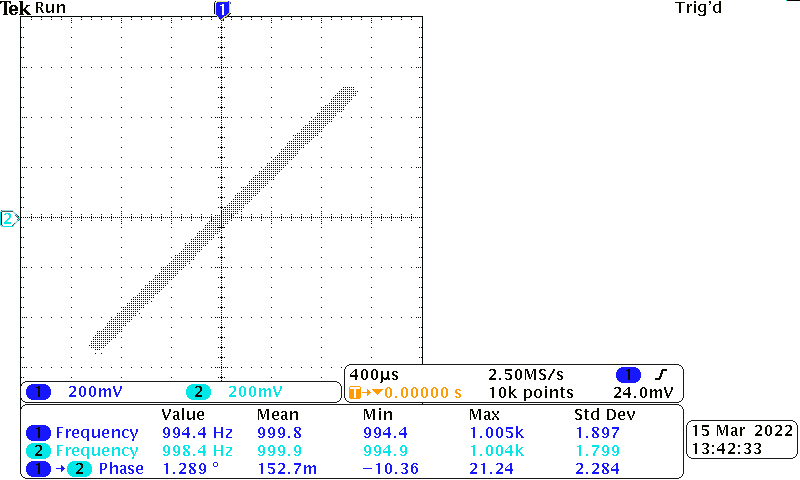
\includegraphics[width=\textwidth]{include/2/3.png}
		\caption{Krzywa Lissajous dla częstotliwości \(f_1=f_2=1\text{kHz}\) i fazie \(\phi=0^{\circ}\)}
	\end{figure}

	\begin{figure}[htp]
		\centering
		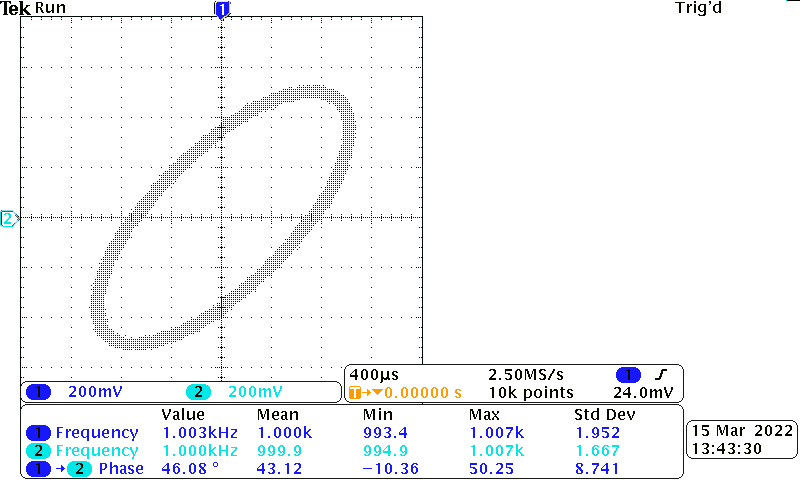
\includegraphics[width=\textwidth]{include/2/4.png}
		\caption{Krzywa Lissajous dla częstotliwości \(f_1=f_2=1\text{kHz}\) i fazie \(\phi=45^{\circ}\)}
	\end{figure}

	\begin{figure}[htp]
		\centering
		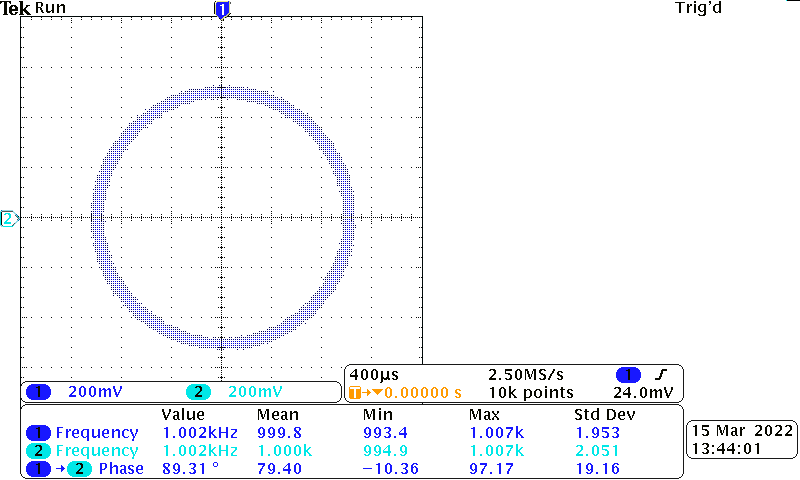
\includegraphics[width=\textwidth]{include/2/5.png}
		\caption{Krzywa Lissajous dla częstotliwości \(f_1=f_2=1\text{kHz}\) i fazie \(\phi=90^{\circ}\)}
	\end{figure}

	\begin{figure}[htp]
		\centering
		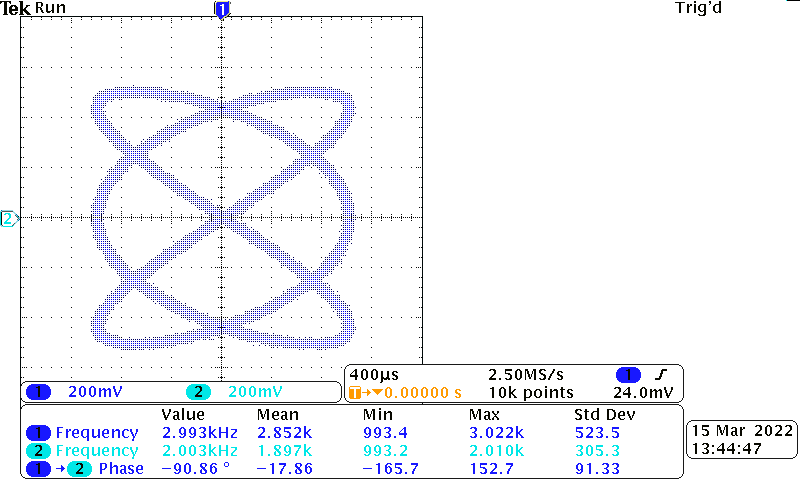
\includegraphics[width=\textwidth]{include/2/6.png}
		\caption{Krzywa Lissajous dla częstotliwości \(f_1=2\text{kHz}\), \(f_2=3\text{kHz}\) i fazie \(\phi=0^{\circ}\)}
	\end{figure}

	\begin{figure}[htp]
		\centering
		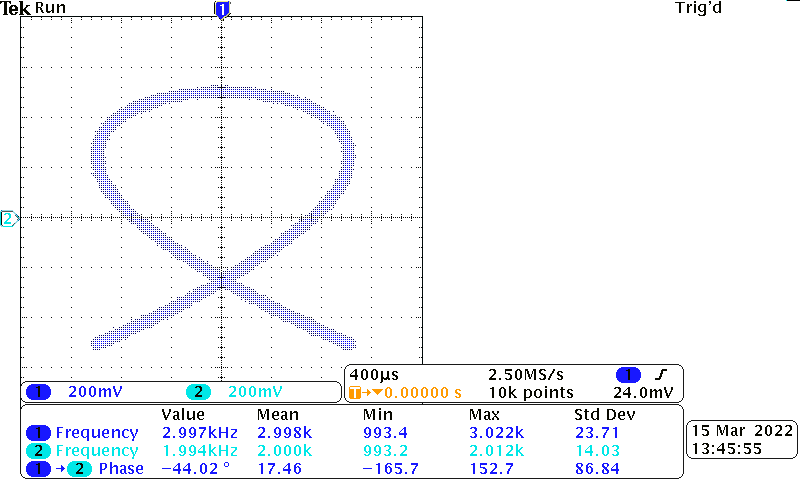
\includegraphics[width=\textwidth]{include/2/7.png}
		\caption{Krzywa Lissajous dla częstotliwości \(f_1=2\text{kHz}\), \(f_2=3\text{kHz}\) i fazie \(\phi=45^{\circ}\)}
	\end{figure}

	\clearpage 
	\section{}
	Wykonano sumowanie dwóch sygnałów sinusoidalnych o częstotliwościach \(f_1=1000\text{Hz}\) i \(f_2=1050\text{Hz}\) i jednakowych amplitudach \(A\).

	\begin{align}
		v_1 = A sin(\omega_1t), \qquad v_2 = A sin(\omega_2t) \\[10pt]
		v = v_1 + v_2 = 2A\;sin(\omega_1t) + sin(\omega_2t) \\[10pt]
		v = 2A\;
		cos \biggl(\frac{\omega_1t-\omega_2t}{2}\biggr)
		sin \biggl(\frac{\omega_1t+\omega_2t}{2}\biggr)
	\end{align}
	\begin{align}
		\text{niech pulsacja dudnień:} &&
		\quad \omega_d &= \frac	
		{\omega_1t-\omega_2t}{2} \\
		\text{natomiast pulsacja wypadkowa:} &&
		\quad \omega_w &= \frac{\omega_1t+\omega_2t}{2} \\
		\text{otrzymujemy:} &&
		\quad v &= a(t)\;sin(\omega_wt) \quad \text{gdzie} \quad a(t) = 2A\;cos(\omega_dt)
	\end{align}

	Podstawiając \(f_1\) i \(f_2\) otrzymujemy \(f_d=25\text{Hz}\).
	Na rysunku poniżej zmierzono czas odpowiadający połowie okresu dudnień, otrzymano w ten sposób dwa razy większą częstotliwość tj. \(50\text{Hz}\).
	Wynik zgadza się z obliczeniami teoretycznymi.

	\begin{figure}[htp]
		\centering
		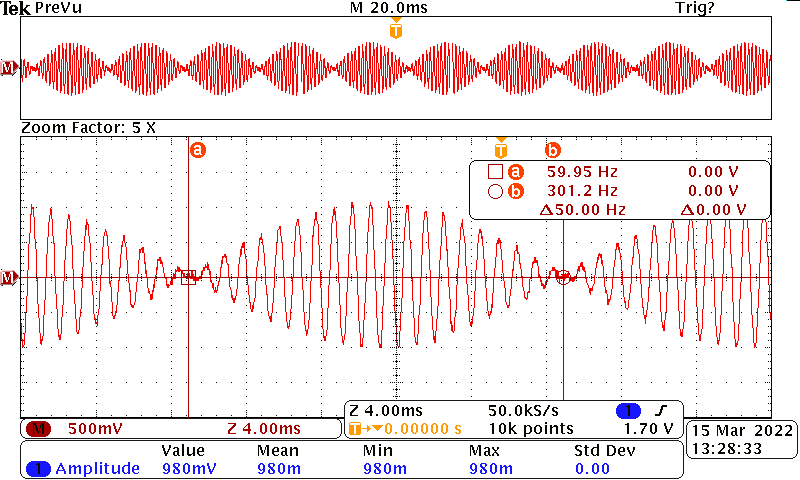
\includegraphics[width=\textwidth]{include/3/1.png}
		\caption{Pomiar połowy okresu oscylacji amplitudy dudnień}
	\end{figure}

	\clearpage
	\section{}
	Zbudowano dzielnik napięcia składający się z dwóch rezystorów \(R_1\) i \(R_2\).
	Wykonano pomiary rezystancji \(R_1\) i \(R_2\) oraz pomiary \(U_{wy}\) dla zadanych wartości \(U_{we} = 1V, 2V, ... , 10V\) przy ustalonej częstotliwości \(f=6\text{kHz}\).
	Zmierzone wartości przedstawiono na wykresie, dokonano regresji liniowej celem znalezienia współczynnika proporcjonalności i porównano go z obliczonym teoretycznie.

	\begin{align}
		U_{wy} = \frac{R_2}{R_1+R_2}\;U_{we} = a\;U_{we}
		\quad \text{gdzie}\;a\;\text{to współczynnik proporcjonalności:}
	\end{align}

	\begin{figure}[htp]
		\centering
		\begin{circuitikz}[european] \draw
			(0,4) node[anchor=east] {$U_{we}$}
			(0,4) to [short, *-] (2,4)
			(4,2) node[anchor=west] {$U_{wy}$}
			(4,2) to [short, *-*] (2,2)

			(2,0) node[ground](GND){} 
			(2,0) to[R, l=$R_2$] (2,2)
			(2,2) to[R, l=$R_1$] (2,4)
			;
		\end{circuitikz}
		\caption{Schemat dzielnika napięcia}
	\end{figure}

	\begin{table}[htp]
		\centering
		\begin{tabular}{c|c|c}
			\hline
			& Znamionowa [k\(\Omega\)] & Zmierzona [k\(\Omega\)] \\ \hline\hline
			\(R_1\) & 0.620 & 0.625 \\ \hline
			\(R_2\) & 3.600 & 3.525 \\ \hline
		\end{tabular}
		\caption{Wartości rezystancji}
	\end{table}

	\begin{table}[htp]
		\centering
		\begin{tabular}{c|c|c}
			\hline
			Zadane \(U_{we}\) [V] & Zmierzone \(U_{we}\) [V] & Zmierzone \(U_{wy}\) [V]
			\\ \hline\hline
			1 & 0.993 & 0.844 \\ \hline
			2 & 1.981 & 1.680 \\ \hline
			3 & 2.940 & 2.504 \\ \hline
			4 & 3.920 & 3.320 \\ \hline
			5 & 4.881 & 4.149 \\ \hline
			6 & 5.846 & 4.960 \\ \hline
			7 & 6.908 & 5.823 \\ \hline
			8 & 7.920 & 6.642 \\ \hline
			9 & 8.880 & 7.520 \\ \hline
			10 & 9.840 & 8.400 \\ \hline
		\end{tabular}
		\caption{Pomiar napięcia wejściowego oraz wyjściowego dzielnika dla zadanego za pomocą generatora napięcia wejściowego}
	\end{table}

	\begin{figure}[htp]
		\centering
		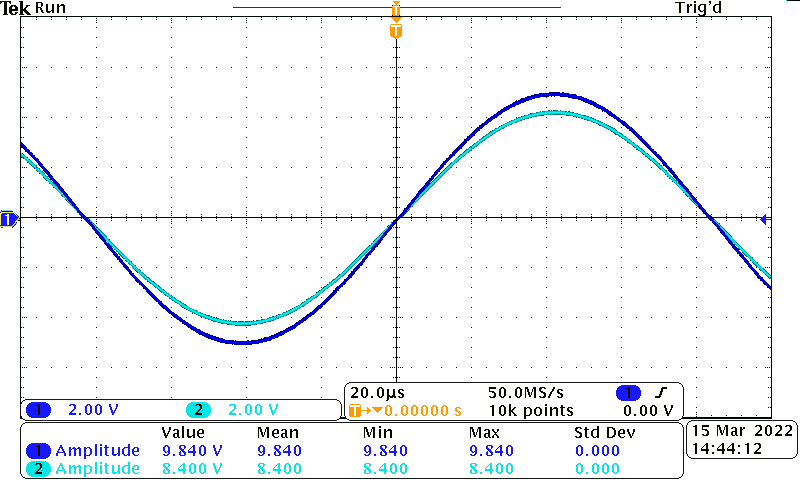
\includegraphics[width=\textwidth]{include/4/10V.png}
		\caption{
			Pomiar napięcia wejściowego oraz wyjściowego dzielnika dla zadanego \(U_{we} = 10V\).
			Analogiczne zostały przeprowadzone dla pozostałych wartości \(U_we\)
		}
	\end{figure}

	\begin{figure}[htp]
		\centering
		%% Creator: Matplotlib, PGF backend
%%
%% To include the figure in your LaTeX document, write
%%   \input{<filename>.pgf}
%%
%% Make sure the required packages are loaded in your preamble
%%   \usepackage{pgf}
%%
%% Also ensure that all the required font packages are loaded; for instance,
%% the lmodern package is sometimes necessary when using math font.
%%   \usepackage{lmodern}
%%
%% Figures using additional raster images can only be included by \input if
%% they are in the same directory as the main LaTeX file. For loading figures
%% from other directories you can use the `import` package
%%   \usepackage{import}
%%
%% and then include the figures with
%%   \import{<path to file>}{<filename>.pgf}
%%
%% Matplotlib used the following preamble
%%
\begingroup%
\makeatletter%
\begin{pgfpicture}%
\pgfpathrectangle{\pgfpointorigin}{\pgfqpoint{6.000000in}{3.750000in}}%
\pgfusepath{use as bounding box, clip}%
\begin{pgfscope}%
\pgfsetbuttcap%
\pgfsetmiterjoin%
\definecolor{currentfill}{rgb}{1.000000,1.000000,1.000000}%
\pgfsetfillcolor{currentfill}%
\pgfsetlinewidth{0.000000pt}%
\definecolor{currentstroke}{rgb}{1.000000,1.000000,1.000000}%
\pgfsetstrokecolor{currentstroke}%
\pgfsetdash{}{0pt}%
\pgfpathmoveto{\pgfqpoint{0.000000in}{0.000000in}}%
\pgfpathlineto{\pgfqpoint{6.000000in}{0.000000in}}%
\pgfpathlineto{\pgfqpoint{6.000000in}{3.750000in}}%
\pgfpathlineto{\pgfqpoint{0.000000in}{3.750000in}}%
\pgfpathlineto{\pgfqpoint{0.000000in}{0.000000in}}%
\pgfpathclose%
\pgfusepath{fill}%
\end{pgfscope}%
\begin{pgfscope}%
\pgfsetbuttcap%
\pgfsetmiterjoin%
\definecolor{currentfill}{rgb}{1.000000,1.000000,1.000000}%
\pgfsetfillcolor{currentfill}%
\pgfsetlinewidth{0.000000pt}%
\definecolor{currentstroke}{rgb}{0.000000,0.000000,0.000000}%
\pgfsetstrokecolor{currentstroke}%
\pgfsetstrokeopacity{0.000000}%
\pgfsetdash{}{0pt}%
\pgfpathmoveto{\pgfqpoint{0.750000in}{0.412500in}}%
\pgfpathlineto{\pgfqpoint{5.400000in}{0.412500in}}%
\pgfpathlineto{\pgfqpoint{5.400000in}{3.300000in}}%
\pgfpathlineto{\pgfqpoint{0.750000in}{3.300000in}}%
\pgfpathlineto{\pgfqpoint{0.750000in}{0.412500in}}%
\pgfpathclose%
\pgfusepath{fill}%
\end{pgfscope}%
\begin{pgfscope}%
\pgfpathrectangle{\pgfqpoint{0.750000in}{0.412500in}}{\pgfqpoint{4.650000in}{2.887500in}}%
\pgfusepath{clip}%
\pgfsetrectcap%
\pgfsetroundjoin%
\pgfsetlinewidth{0.803000pt}%
\definecolor{currentstroke}{rgb}{0.690196,0.690196,0.690196}%
\pgfsetstrokecolor{currentstroke}%
\pgfsetdash{}{0pt}%
\pgfpathmoveto{\pgfqpoint{0.961364in}{0.412500in}}%
\pgfpathlineto{\pgfqpoint{0.961364in}{3.300000in}}%
\pgfusepath{stroke}%
\end{pgfscope}%
\begin{pgfscope}%
\pgfsetbuttcap%
\pgfsetroundjoin%
\definecolor{currentfill}{rgb}{0.000000,0.000000,0.000000}%
\pgfsetfillcolor{currentfill}%
\pgfsetlinewidth{0.803000pt}%
\definecolor{currentstroke}{rgb}{0.000000,0.000000,0.000000}%
\pgfsetstrokecolor{currentstroke}%
\pgfsetdash{}{0pt}%
\pgfsys@defobject{currentmarker}{\pgfqpoint{0.000000in}{-0.048611in}}{\pgfqpoint{0.000000in}{0.000000in}}{%
\pgfpathmoveto{\pgfqpoint{0.000000in}{0.000000in}}%
\pgfpathlineto{\pgfqpoint{0.000000in}{-0.048611in}}%
\pgfusepath{stroke,fill}%
}%
\begin{pgfscope}%
\pgfsys@transformshift{0.961364in}{0.412500in}%
\pgfsys@useobject{currentmarker}{}%
\end{pgfscope}%
\end{pgfscope}%
\begin{pgfscope}%
\definecolor{textcolor}{rgb}{0.000000,0.000000,0.000000}%
\pgfsetstrokecolor{textcolor}%
\pgfsetfillcolor{textcolor}%
\pgftext[x=0.961364in,y=0.315278in,,top]{\color{textcolor}\rmfamily\fontsize{10.000000}{12.000000}\selectfont \(\displaystyle {0}\)}%
\end{pgfscope}%
\begin{pgfscope}%
\pgfpathrectangle{\pgfqpoint{0.750000in}{0.412500in}}{\pgfqpoint{4.650000in}{2.887500in}}%
\pgfusepath{clip}%
\pgfsetrectcap%
\pgfsetroundjoin%
\pgfsetlinewidth{0.803000pt}%
\definecolor{currentstroke}{rgb}{0.690196,0.690196,0.690196}%
\pgfsetstrokecolor{currentstroke}%
\pgfsetdash{}{0pt}%
\pgfpathmoveto{\pgfqpoint{1.806818in}{0.412500in}}%
\pgfpathlineto{\pgfqpoint{1.806818in}{3.300000in}}%
\pgfusepath{stroke}%
\end{pgfscope}%
\begin{pgfscope}%
\pgfsetbuttcap%
\pgfsetroundjoin%
\definecolor{currentfill}{rgb}{0.000000,0.000000,0.000000}%
\pgfsetfillcolor{currentfill}%
\pgfsetlinewidth{0.803000pt}%
\definecolor{currentstroke}{rgb}{0.000000,0.000000,0.000000}%
\pgfsetstrokecolor{currentstroke}%
\pgfsetdash{}{0pt}%
\pgfsys@defobject{currentmarker}{\pgfqpoint{0.000000in}{-0.048611in}}{\pgfqpoint{0.000000in}{0.000000in}}{%
\pgfpathmoveto{\pgfqpoint{0.000000in}{0.000000in}}%
\pgfpathlineto{\pgfqpoint{0.000000in}{-0.048611in}}%
\pgfusepath{stroke,fill}%
}%
\begin{pgfscope}%
\pgfsys@transformshift{1.806818in}{0.412500in}%
\pgfsys@useobject{currentmarker}{}%
\end{pgfscope}%
\end{pgfscope}%
\begin{pgfscope}%
\definecolor{textcolor}{rgb}{0.000000,0.000000,0.000000}%
\pgfsetstrokecolor{textcolor}%
\pgfsetfillcolor{textcolor}%
\pgftext[x=1.806818in,y=0.315278in,,top]{\color{textcolor}\rmfamily\fontsize{10.000000}{12.000000}\selectfont \(\displaystyle {2}\)}%
\end{pgfscope}%
\begin{pgfscope}%
\pgfpathrectangle{\pgfqpoint{0.750000in}{0.412500in}}{\pgfqpoint{4.650000in}{2.887500in}}%
\pgfusepath{clip}%
\pgfsetrectcap%
\pgfsetroundjoin%
\pgfsetlinewidth{0.803000pt}%
\definecolor{currentstroke}{rgb}{0.690196,0.690196,0.690196}%
\pgfsetstrokecolor{currentstroke}%
\pgfsetdash{}{0pt}%
\pgfpathmoveto{\pgfqpoint{2.652273in}{0.412500in}}%
\pgfpathlineto{\pgfqpoint{2.652273in}{3.300000in}}%
\pgfusepath{stroke}%
\end{pgfscope}%
\begin{pgfscope}%
\pgfsetbuttcap%
\pgfsetroundjoin%
\definecolor{currentfill}{rgb}{0.000000,0.000000,0.000000}%
\pgfsetfillcolor{currentfill}%
\pgfsetlinewidth{0.803000pt}%
\definecolor{currentstroke}{rgb}{0.000000,0.000000,0.000000}%
\pgfsetstrokecolor{currentstroke}%
\pgfsetdash{}{0pt}%
\pgfsys@defobject{currentmarker}{\pgfqpoint{0.000000in}{-0.048611in}}{\pgfqpoint{0.000000in}{0.000000in}}{%
\pgfpathmoveto{\pgfqpoint{0.000000in}{0.000000in}}%
\pgfpathlineto{\pgfqpoint{0.000000in}{-0.048611in}}%
\pgfusepath{stroke,fill}%
}%
\begin{pgfscope}%
\pgfsys@transformshift{2.652273in}{0.412500in}%
\pgfsys@useobject{currentmarker}{}%
\end{pgfscope}%
\end{pgfscope}%
\begin{pgfscope}%
\definecolor{textcolor}{rgb}{0.000000,0.000000,0.000000}%
\pgfsetstrokecolor{textcolor}%
\pgfsetfillcolor{textcolor}%
\pgftext[x=2.652273in,y=0.315278in,,top]{\color{textcolor}\rmfamily\fontsize{10.000000}{12.000000}\selectfont \(\displaystyle {4}\)}%
\end{pgfscope}%
\begin{pgfscope}%
\pgfpathrectangle{\pgfqpoint{0.750000in}{0.412500in}}{\pgfqpoint{4.650000in}{2.887500in}}%
\pgfusepath{clip}%
\pgfsetrectcap%
\pgfsetroundjoin%
\pgfsetlinewidth{0.803000pt}%
\definecolor{currentstroke}{rgb}{0.690196,0.690196,0.690196}%
\pgfsetstrokecolor{currentstroke}%
\pgfsetdash{}{0pt}%
\pgfpathmoveto{\pgfqpoint{3.497727in}{0.412500in}}%
\pgfpathlineto{\pgfqpoint{3.497727in}{3.300000in}}%
\pgfusepath{stroke}%
\end{pgfscope}%
\begin{pgfscope}%
\pgfsetbuttcap%
\pgfsetroundjoin%
\definecolor{currentfill}{rgb}{0.000000,0.000000,0.000000}%
\pgfsetfillcolor{currentfill}%
\pgfsetlinewidth{0.803000pt}%
\definecolor{currentstroke}{rgb}{0.000000,0.000000,0.000000}%
\pgfsetstrokecolor{currentstroke}%
\pgfsetdash{}{0pt}%
\pgfsys@defobject{currentmarker}{\pgfqpoint{0.000000in}{-0.048611in}}{\pgfqpoint{0.000000in}{0.000000in}}{%
\pgfpathmoveto{\pgfqpoint{0.000000in}{0.000000in}}%
\pgfpathlineto{\pgfqpoint{0.000000in}{-0.048611in}}%
\pgfusepath{stroke,fill}%
}%
\begin{pgfscope}%
\pgfsys@transformshift{3.497727in}{0.412500in}%
\pgfsys@useobject{currentmarker}{}%
\end{pgfscope}%
\end{pgfscope}%
\begin{pgfscope}%
\definecolor{textcolor}{rgb}{0.000000,0.000000,0.000000}%
\pgfsetstrokecolor{textcolor}%
\pgfsetfillcolor{textcolor}%
\pgftext[x=3.497727in,y=0.315278in,,top]{\color{textcolor}\rmfamily\fontsize{10.000000}{12.000000}\selectfont \(\displaystyle {6}\)}%
\end{pgfscope}%
\begin{pgfscope}%
\pgfpathrectangle{\pgfqpoint{0.750000in}{0.412500in}}{\pgfqpoint{4.650000in}{2.887500in}}%
\pgfusepath{clip}%
\pgfsetrectcap%
\pgfsetroundjoin%
\pgfsetlinewidth{0.803000pt}%
\definecolor{currentstroke}{rgb}{0.690196,0.690196,0.690196}%
\pgfsetstrokecolor{currentstroke}%
\pgfsetdash{}{0pt}%
\pgfpathmoveto{\pgfqpoint{4.343182in}{0.412500in}}%
\pgfpathlineto{\pgfqpoint{4.343182in}{3.300000in}}%
\pgfusepath{stroke}%
\end{pgfscope}%
\begin{pgfscope}%
\pgfsetbuttcap%
\pgfsetroundjoin%
\definecolor{currentfill}{rgb}{0.000000,0.000000,0.000000}%
\pgfsetfillcolor{currentfill}%
\pgfsetlinewidth{0.803000pt}%
\definecolor{currentstroke}{rgb}{0.000000,0.000000,0.000000}%
\pgfsetstrokecolor{currentstroke}%
\pgfsetdash{}{0pt}%
\pgfsys@defobject{currentmarker}{\pgfqpoint{0.000000in}{-0.048611in}}{\pgfqpoint{0.000000in}{0.000000in}}{%
\pgfpathmoveto{\pgfqpoint{0.000000in}{0.000000in}}%
\pgfpathlineto{\pgfqpoint{0.000000in}{-0.048611in}}%
\pgfusepath{stroke,fill}%
}%
\begin{pgfscope}%
\pgfsys@transformshift{4.343182in}{0.412500in}%
\pgfsys@useobject{currentmarker}{}%
\end{pgfscope}%
\end{pgfscope}%
\begin{pgfscope}%
\definecolor{textcolor}{rgb}{0.000000,0.000000,0.000000}%
\pgfsetstrokecolor{textcolor}%
\pgfsetfillcolor{textcolor}%
\pgftext[x=4.343182in,y=0.315278in,,top]{\color{textcolor}\rmfamily\fontsize{10.000000}{12.000000}\selectfont \(\displaystyle {8}\)}%
\end{pgfscope}%
\begin{pgfscope}%
\pgfpathrectangle{\pgfqpoint{0.750000in}{0.412500in}}{\pgfqpoint{4.650000in}{2.887500in}}%
\pgfusepath{clip}%
\pgfsetrectcap%
\pgfsetroundjoin%
\pgfsetlinewidth{0.803000pt}%
\definecolor{currentstroke}{rgb}{0.690196,0.690196,0.690196}%
\pgfsetstrokecolor{currentstroke}%
\pgfsetdash{}{0pt}%
\pgfpathmoveto{\pgfqpoint{5.188636in}{0.412500in}}%
\pgfpathlineto{\pgfqpoint{5.188636in}{3.300000in}}%
\pgfusepath{stroke}%
\end{pgfscope}%
\begin{pgfscope}%
\pgfsetbuttcap%
\pgfsetroundjoin%
\definecolor{currentfill}{rgb}{0.000000,0.000000,0.000000}%
\pgfsetfillcolor{currentfill}%
\pgfsetlinewidth{0.803000pt}%
\definecolor{currentstroke}{rgb}{0.000000,0.000000,0.000000}%
\pgfsetstrokecolor{currentstroke}%
\pgfsetdash{}{0pt}%
\pgfsys@defobject{currentmarker}{\pgfqpoint{0.000000in}{-0.048611in}}{\pgfqpoint{0.000000in}{0.000000in}}{%
\pgfpathmoveto{\pgfqpoint{0.000000in}{0.000000in}}%
\pgfpathlineto{\pgfqpoint{0.000000in}{-0.048611in}}%
\pgfusepath{stroke,fill}%
}%
\begin{pgfscope}%
\pgfsys@transformshift{5.188636in}{0.412500in}%
\pgfsys@useobject{currentmarker}{}%
\end{pgfscope}%
\end{pgfscope}%
\begin{pgfscope}%
\definecolor{textcolor}{rgb}{0.000000,0.000000,0.000000}%
\pgfsetstrokecolor{textcolor}%
\pgfsetfillcolor{textcolor}%
\pgftext[x=5.188636in,y=0.315278in,,top]{\color{textcolor}\rmfamily\fontsize{10.000000}{12.000000}\selectfont \(\displaystyle {10}\)}%
\end{pgfscope}%
\begin{pgfscope}%
\definecolor{textcolor}{rgb}{0.000000,0.000000,0.000000}%
\pgfsetstrokecolor{textcolor}%
\pgfsetfillcolor{textcolor}%
\pgftext[x=3.075000in,y=0.136266in,,top]{\color{textcolor}\rmfamily\fontsize{10.000000}{12.000000}\selectfont \(\displaystyle U_{we}\)}%
\end{pgfscope}%
\begin{pgfscope}%
\pgfpathrectangle{\pgfqpoint{0.750000in}{0.412500in}}{\pgfqpoint{4.650000in}{2.887500in}}%
\pgfusepath{clip}%
\pgfsetrectcap%
\pgfsetroundjoin%
\pgfsetlinewidth{0.803000pt}%
\definecolor{currentstroke}{rgb}{0.690196,0.690196,0.690196}%
\pgfsetstrokecolor{currentstroke}%
\pgfsetdash{}{0pt}%
\pgfpathmoveto{\pgfqpoint{0.750000in}{0.543750in}}%
\pgfpathlineto{\pgfqpoint{5.400000in}{0.543750in}}%
\pgfusepath{stroke}%
\end{pgfscope}%
\begin{pgfscope}%
\pgfsetbuttcap%
\pgfsetroundjoin%
\definecolor{currentfill}{rgb}{0.000000,0.000000,0.000000}%
\pgfsetfillcolor{currentfill}%
\pgfsetlinewidth{0.803000pt}%
\definecolor{currentstroke}{rgb}{0.000000,0.000000,0.000000}%
\pgfsetstrokecolor{currentstroke}%
\pgfsetdash{}{0pt}%
\pgfsys@defobject{currentmarker}{\pgfqpoint{-0.048611in}{0.000000in}}{\pgfqpoint{-0.000000in}{0.000000in}}{%
\pgfpathmoveto{\pgfqpoint{-0.000000in}{0.000000in}}%
\pgfpathlineto{\pgfqpoint{-0.048611in}{0.000000in}}%
\pgfusepath{stroke,fill}%
}%
\begin{pgfscope}%
\pgfsys@transformshift{0.750000in}{0.543750in}%
\pgfsys@useobject{currentmarker}{}%
\end{pgfscope}%
\end{pgfscope}%
\begin{pgfscope}%
\definecolor{textcolor}{rgb}{0.000000,0.000000,0.000000}%
\pgfsetstrokecolor{textcolor}%
\pgfsetfillcolor{textcolor}%
\pgftext[x=0.583333in, y=0.495525in, left, base]{\color{textcolor}\rmfamily\fontsize{10.000000}{12.000000}\selectfont \(\displaystyle {0}\)}%
\end{pgfscope}%
\begin{pgfscope}%
\pgfpathrectangle{\pgfqpoint{0.750000in}{0.412500in}}{\pgfqpoint{4.650000in}{2.887500in}}%
\pgfusepath{clip}%
\pgfsetrectcap%
\pgfsetroundjoin%
\pgfsetlinewidth{0.803000pt}%
\definecolor{currentstroke}{rgb}{0.690196,0.690196,0.690196}%
\pgfsetstrokecolor{currentstroke}%
\pgfsetdash{}{0pt}%
\pgfpathmoveto{\pgfqpoint{0.750000in}{1.163423in}}%
\pgfpathlineto{\pgfqpoint{5.400000in}{1.163423in}}%
\pgfusepath{stroke}%
\end{pgfscope}%
\begin{pgfscope}%
\pgfsetbuttcap%
\pgfsetroundjoin%
\definecolor{currentfill}{rgb}{0.000000,0.000000,0.000000}%
\pgfsetfillcolor{currentfill}%
\pgfsetlinewidth{0.803000pt}%
\definecolor{currentstroke}{rgb}{0.000000,0.000000,0.000000}%
\pgfsetstrokecolor{currentstroke}%
\pgfsetdash{}{0pt}%
\pgfsys@defobject{currentmarker}{\pgfqpoint{-0.048611in}{0.000000in}}{\pgfqpoint{-0.000000in}{0.000000in}}{%
\pgfpathmoveto{\pgfqpoint{-0.000000in}{0.000000in}}%
\pgfpathlineto{\pgfqpoint{-0.048611in}{0.000000in}}%
\pgfusepath{stroke,fill}%
}%
\begin{pgfscope}%
\pgfsys@transformshift{0.750000in}{1.163423in}%
\pgfsys@useobject{currentmarker}{}%
\end{pgfscope}%
\end{pgfscope}%
\begin{pgfscope}%
\definecolor{textcolor}{rgb}{0.000000,0.000000,0.000000}%
\pgfsetstrokecolor{textcolor}%
\pgfsetfillcolor{textcolor}%
\pgftext[x=0.583333in, y=1.115198in, left, base]{\color{textcolor}\rmfamily\fontsize{10.000000}{12.000000}\selectfont \(\displaystyle {2}\)}%
\end{pgfscope}%
\begin{pgfscope}%
\pgfpathrectangle{\pgfqpoint{0.750000in}{0.412500in}}{\pgfqpoint{4.650000in}{2.887500in}}%
\pgfusepath{clip}%
\pgfsetrectcap%
\pgfsetroundjoin%
\pgfsetlinewidth{0.803000pt}%
\definecolor{currentstroke}{rgb}{0.690196,0.690196,0.690196}%
\pgfsetstrokecolor{currentstroke}%
\pgfsetdash{}{0pt}%
\pgfpathmoveto{\pgfqpoint{0.750000in}{1.783096in}}%
\pgfpathlineto{\pgfqpoint{5.400000in}{1.783096in}}%
\pgfusepath{stroke}%
\end{pgfscope}%
\begin{pgfscope}%
\pgfsetbuttcap%
\pgfsetroundjoin%
\definecolor{currentfill}{rgb}{0.000000,0.000000,0.000000}%
\pgfsetfillcolor{currentfill}%
\pgfsetlinewidth{0.803000pt}%
\definecolor{currentstroke}{rgb}{0.000000,0.000000,0.000000}%
\pgfsetstrokecolor{currentstroke}%
\pgfsetdash{}{0pt}%
\pgfsys@defobject{currentmarker}{\pgfqpoint{-0.048611in}{0.000000in}}{\pgfqpoint{-0.000000in}{0.000000in}}{%
\pgfpathmoveto{\pgfqpoint{-0.000000in}{0.000000in}}%
\pgfpathlineto{\pgfqpoint{-0.048611in}{0.000000in}}%
\pgfusepath{stroke,fill}%
}%
\begin{pgfscope}%
\pgfsys@transformshift{0.750000in}{1.783096in}%
\pgfsys@useobject{currentmarker}{}%
\end{pgfscope}%
\end{pgfscope}%
\begin{pgfscope}%
\definecolor{textcolor}{rgb}{0.000000,0.000000,0.000000}%
\pgfsetstrokecolor{textcolor}%
\pgfsetfillcolor{textcolor}%
\pgftext[x=0.583333in, y=1.734871in, left, base]{\color{textcolor}\rmfamily\fontsize{10.000000}{12.000000}\selectfont \(\displaystyle {4}\)}%
\end{pgfscope}%
\begin{pgfscope}%
\pgfpathrectangle{\pgfqpoint{0.750000in}{0.412500in}}{\pgfqpoint{4.650000in}{2.887500in}}%
\pgfusepath{clip}%
\pgfsetrectcap%
\pgfsetroundjoin%
\pgfsetlinewidth{0.803000pt}%
\definecolor{currentstroke}{rgb}{0.690196,0.690196,0.690196}%
\pgfsetstrokecolor{currentstroke}%
\pgfsetdash{}{0pt}%
\pgfpathmoveto{\pgfqpoint{0.750000in}{2.402770in}}%
\pgfpathlineto{\pgfqpoint{5.400000in}{2.402770in}}%
\pgfusepath{stroke}%
\end{pgfscope}%
\begin{pgfscope}%
\pgfsetbuttcap%
\pgfsetroundjoin%
\definecolor{currentfill}{rgb}{0.000000,0.000000,0.000000}%
\pgfsetfillcolor{currentfill}%
\pgfsetlinewidth{0.803000pt}%
\definecolor{currentstroke}{rgb}{0.000000,0.000000,0.000000}%
\pgfsetstrokecolor{currentstroke}%
\pgfsetdash{}{0pt}%
\pgfsys@defobject{currentmarker}{\pgfqpoint{-0.048611in}{0.000000in}}{\pgfqpoint{-0.000000in}{0.000000in}}{%
\pgfpathmoveto{\pgfqpoint{-0.000000in}{0.000000in}}%
\pgfpathlineto{\pgfqpoint{-0.048611in}{0.000000in}}%
\pgfusepath{stroke,fill}%
}%
\begin{pgfscope}%
\pgfsys@transformshift{0.750000in}{2.402770in}%
\pgfsys@useobject{currentmarker}{}%
\end{pgfscope}%
\end{pgfscope}%
\begin{pgfscope}%
\definecolor{textcolor}{rgb}{0.000000,0.000000,0.000000}%
\pgfsetstrokecolor{textcolor}%
\pgfsetfillcolor{textcolor}%
\pgftext[x=0.583333in, y=2.354544in, left, base]{\color{textcolor}\rmfamily\fontsize{10.000000}{12.000000}\selectfont \(\displaystyle {6}\)}%
\end{pgfscope}%
\begin{pgfscope}%
\pgfpathrectangle{\pgfqpoint{0.750000in}{0.412500in}}{\pgfqpoint{4.650000in}{2.887500in}}%
\pgfusepath{clip}%
\pgfsetrectcap%
\pgfsetroundjoin%
\pgfsetlinewidth{0.803000pt}%
\definecolor{currentstroke}{rgb}{0.690196,0.690196,0.690196}%
\pgfsetstrokecolor{currentstroke}%
\pgfsetdash{}{0pt}%
\pgfpathmoveto{\pgfqpoint{0.750000in}{3.022443in}}%
\pgfpathlineto{\pgfqpoint{5.400000in}{3.022443in}}%
\pgfusepath{stroke}%
\end{pgfscope}%
\begin{pgfscope}%
\pgfsetbuttcap%
\pgfsetroundjoin%
\definecolor{currentfill}{rgb}{0.000000,0.000000,0.000000}%
\pgfsetfillcolor{currentfill}%
\pgfsetlinewidth{0.803000pt}%
\definecolor{currentstroke}{rgb}{0.000000,0.000000,0.000000}%
\pgfsetstrokecolor{currentstroke}%
\pgfsetdash{}{0pt}%
\pgfsys@defobject{currentmarker}{\pgfqpoint{-0.048611in}{0.000000in}}{\pgfqpoint{-0.000000in}{0.000000in}}{%
\pgfpathmoveto{\pgfqpoint{-0.000000in}{0.000000in}}%
\pgfpathlineto{\pgfqpoint{-0.048611in}{0.000000in}}%
\pgfusepath{stroke,fill}%
}%
\begin{pgfscope}%
\pgfsys@transformshift{0.750000in}{3.022443in}%
\pgfsys@useobject{currentmarker}{}%
\end{pgfscope}%
\end{pgfscope}%
\begin{pgfscope}%
\definecolor{textcolor}{rgb}{0.000000,0.000000,0.000000}%
\pgfsetstrokecolor{textcolor}%
\pgfsetfillcolor{textcolor}%
\pgftext[x=0.583333in, y=2.974218in, left, base]{\color{textcolor}\rmfamily\fontsize{10.000000}{12.000000}\selectfont \(\displaystyle {8}\)}%
\end{pgfscope}%
\begin{pgfscope}%
\definecolor{textcolor}{rgb}{0.000000,0.000000,0.000000}%
\pgfsetstrokecolor{textcolor}%
\pgfsetfillcolor{textcolor}%
\pgftext[x=0.527778in,y=1.856250in,,bottom,rotate=90.000000]{\color{textcolor}\rmfamily\fontsize{10.000000}{12.000000}\selectfont \(\displaystyle U_{wy}\)}%
\end{pgfscope}%
\begin{pgfscope}%
\pgfpathrectangle{\pgfqpoint{0.750000in}{0.412500in}}{\pgfqpoint{4.650000in}{2.887500in}}%
\pgfusepath{clip}%
\pgfsetrectcap%
\pgfsetroundjoin%
\pgfsetlinewidth{1.505625pt}%
\definecolor{currentstroke}{rgb}{0.121569,0.466667,0.705882}%
\pgfsetstrokecolor{currentstroke}%
\pgfsetdash{}{0pt}%
\pgfpathmoveto{\pgfqpoint{0.961364in}{0.543750in}}%
\pgfpathlineto{\pgfqpoint{1.047635in}{0.597321in}}%
\pgfpathlineto{\pgfqpoint{1.133905in}{0.650893in}}%
\pgfpathlineto{\pgfqpoint{1.220176in}{0.704464in}}%
\pgfpathlineto{\pgfqpoint{1.306447in}{0.758036in}}%
\pgfpathlineto{\pgfqpoint{1.392718in}{0.811607in}}%
\pgfpathlineto{\pgfqpoint{1.478989in}{0.865179in}}%
\pgfpathlineto{\pgfqpoint{1.565260in}{0.918750in}}%
\pgfpathlineto{\pgfqpoint{1.651531in}{0.972321in}}%
\pgfpathlineto{\pgfqpoint{1.737801in}{1.025893in}}%
\pgfpathlineto{\pgfqpoint{1.824072in}{1.079464in}}%
\pgfpathlineto{\pgfqpoint{1.910343in}{1.133036in}}%
\pgfpathlineto{\pgfqpoint{1.996614in}{1.186607in}}%
\pgfpathlineto{\pgfqpoint{2.082885in}{1.240179in}}%
\pgfpathlineto{\pgfqpoint{2.169156in}{1.293750in}}%
\pgfpathlineto{\pgfqpoint{2.255427in}{1.347321in}}%
\pgfpathlineto{\pgfqpoint{2.341698in}{1.400893in}}%
\pgfpathlineto{\pgfqpoint{2.427968in}{1.454464in}}%
\pgfpathlineto{\pgfqpoint{2.514239in}{1.508036in}}%
\pgfpathlineto{\pgfqpoint{2.600510in}{1.561607in}}%
\pgfpathlineto{\pgfqpoint{2.686781in}{1.615179in}}%
\pgfpathlineto{\pgfqpoint{2.773052in}{1.668750in}}%
\pgfpathlineto{\pgfqpoint{2.859323in}{1.722321in}}%
\pgfpathlineto{\pgfqpoint{2.945594in}{1.775893in}}%
\pgfpathlineto{\pgfqpoint{3.031865in}{1.829464in}}%
\pgfpathlineto{\pgfqpoint{3.118135in}{1.883036in}}%
\pgfpathlineto{\pgfqpoint{3.204406in}{1.936607in}}%
\pgfpathlineto{\pgfqpoint{3.290677in}{1.990179in}}%
\pgfpathlineto{\pgfqpoint{3.376948in}{2.043750in}}%
\pgfpathlineto{\pgfqpoint{3.463219in}{2.097321in}}%
\pgfpathlineto{\pgfqpoint{3.549490in}{2.150893in}}%
\pgfpathlineto{\pgfqpoint{3.635761in}{2.204464in}}%
\pgfpathlineto{\pgfqpoint{3.722032in}{2.258036in}}%
\pgfpathlineto{\pgfqpoint{3.808302in}{2.311607in}}%
\pgfpathlineto{\pgfqpoint{3.894573in}{2.365179in}}%
\pgfpathlineto{\pgfqpoint{3.980844in}{2.418750in}}%
\pgfpathlineto{\pgfqpoint{4.067115in}{2.472321in}}%
\pgfpathlineto{\pgfqpoint{4.153386in}{2.525893in}}%
\pgfpathlineto{\pgfqpoint{4.239657in}{2.579464in}}%
\pgfpathlineto{\pgfqpoint{4.325928in}{2.633036in}}%
\pgfpathlineto{\pgfqpoint{4.412199in}{2.686607in}}%
\pgfpathlineto{\pgfqpoint{4.498469in}{2.740179in}}%
\pgfpathlineto{\pgfqpoint{4.584740in}{2.793750in}}%
\pgfpathlineto{\pgfqpoint{4.671011in}{2.847321in}}%
\pgfpathlineto{\pgfqpoint{4.757282in}{2.900893in}}%
\pgfpathlineto{\pgfqpoint{4.843553in}{2.954464in}}%
\pgfpathlineto{\pgfqpoint{4.929824in}{3.008036in}}%
\pgfpathlineto{\pgfqpoint{5.016095in}{3.061607in}}%
\pgfpathlineto{\pgfqpoint{5.102365in}{3.115179in}}%
\pgfpathlineto{\pgfqpoint{5.188636in}{3.168750in}}%
\pgfusepath{stroke}%
\end{pgfscope}%
\begin{pgfscope}%
\pgfpathrectangle{\pgfqpoint{0.750000in}{0.412500in}}{\pgfqpoint{4.650000in}{2.887500in}}%
\pgfusepath{clip}%
\pgfsetrectcap%
\pgfsetroundjoin%
\pgfsetlinewidth{0.000000pt}%
\definecolor{currentstroke}{rgb}{1.000000,0.498039,0.054902}%
\pgfsetstrokecolor{currentstroke}%
\pgfsetdash{}{0pt}%
\pgfpathmoveto{\pgfqpoint{1.381132in}{0.805252in}}%
\pgfpathlineto{\pgfqpoint{1.798786in}{1.064275in}}%
\pgfpathlineto{\pgfqpoint{2.204182in}{1.319581in}}%
\pgfpathlineto{\pgfqpoint{2.618455in}{1.572408in}}%
\pgfpathlineto{\pgfqpoint{3.024695in}{1.829262in}}%
\pgfpathlineto{\pgfqpoint{3.432627in}{2.080540in}}%
\pgfpathlineto{\pgfqpoint{3.881564in}{2.347929in}}%
\pgfpathlineto{\pgfqpoint{4.309364in}{2.601685in}}%
\pgfpathlineto{\pgfqpoint{4.715182in}{2.873721in}}%
\pgfpathlineto{\pgfqpoint{5.121000in}{3.146377in}}%
\pgfusepath{}%
\end{pgfscope}%
\begin{pgfscope}%
\pgfpathrectangle{\pgfqpoint{0.750000in}{0.412500in}}{\pgfqpoint{4.650000in}{2.887500in}}%
\pgfusepath{clip}%
\pgfsetbuttcap%
\pgfsetroundjoin%
\definecolor{currentfill}{rgb}{1.000000,0.498039,0.054902}%
\pgfsetfillcolor{currentfill}%
\pgfsetlinewidth{1.003750pt}%
\definecolor{currentstroke}{rgb}{1.000000,0.498039,0.054902}%
\pgfsetstrokecolor{currentstroke}%
\pgfsetdash{}{0pt}%
\pgfsys@defobject{currentmarker}{\pgfqpoint{-0.041667in}{-0.041667in}}{\pgfqpoint{0.041667in}{0.041667in}}{%
\pgfpathmoveto{\pgfqpoint{0.000000in}{-0.041667in}}%
\pgfpathcurveto{\pgfqpoint{0.011050in}{-0.041667in}}{\pgfqpoint{0.021649in}{-0.037276in}}{\pgfqpoint{0.029463in}{-0.029463in}}%
\pgfpathcurveto{\pgfqpoint{0.037276in}{-0.021649in}}{\pgfqpoint{0.041667in}{-0.011050in}}{\pgfqpoint{0.041667in}{0.000000in}}%
\pgfpathcurveto{\pgfqpoint{0.041667in}{0.011050in}}{\pgfqpoint{0.037276in}{0.021649in}}{\pgfqpoint{0.029463in}{0.029463in}}%
\pgfpathcurveto{\pgfqpoint{0.021649in}{0.037276in}}{\pgfqpoint{0.011050in}{0.041667in}}{\pgfqpoint{0.000000in}{0.041667in}}%
\pgfpathcurveto{\pgfqpoint{-0.011050in}{0.041667in}}{\pgfqpoint{-0.021649in}{0.037276in}}{\pgfqpoint{-0.029463in}{0.029463in}}%
\pgfpathcurveto{\pgfqpoint{-0.037276in}{0.021649in}}{\pgfqpoint{-0.041667in}{0.011050in}}{\pgfqpoint{-0.041667in}{0.000000in}}%
\pgfpathcurveto{\pgfqpoint{-0.041667in}{-0.011050in}}{\pgfqpoint{-0.037276in}{-0.021649in}}{\pgfqpoint{-0.029463in}{-0.029463in}}%
\pgfpathcurveto{\pgfqpoint{-0.021649in}{-0.037276in}}{\pgfqpoint{-0.011050in}{-0.041667in}}{\pgfqpoint{0.000000in}{-0.041667in}}%
\pgfpathlineto{\pgfqpoint{0.000000in}{-0.041667in}}%
\pgfpathclose%
\pgfusepath{stroke,fill}%
}%
\begin{pgfscope}%
\pgfsys@transformshift{1.381132in}{0.805252in}%
\pgfsys@useobject{currentmarker}{}%
\end{pgfscope}%
\begin{pgfscope}%
\pgfsys@transformshift{1.798786in}{1.064275in}%
\pgfsys@useobject{currentmarker}{}%
\end{pgfscope}%
\begin{pgfscope}%
\pgfsys@transformshift{2.204182in}{1.319581in}%
\pgfsys@useobject{currentmarker}{}%
\end{pgfscope}%
\begin{pgfscope}%
\pgfsys@transformshift{2.618455in}{1.572408in}%
\pgfsys@useobject{currentmarker}{}%
\end{pgfscope}%
\begin{pgfscope}%
\pgfsys@transformshift{3.024695in}{1.829262in}%
\pgfsys@useobject{currentmarker}{}%
\end{pgfscope}%
\begin{pgfscope}%
\pgfsys@transformshift{3.432627in}{2.080540in}%
\pgfsys@useobject{currentmarker}{}%
\end{pgfscope}%
\begin{pgfscope}%
\pgfsys@transformshift{3.881564in}{2.347929in}%
\pgfsys@useobject{currentmarker}{}%
\end{pgfscope}%
\begin{pgfscope}%
\pgfsys@transformshift{4.309364in}{2.601685in}%
\pgfsys@useobject{currentmarker}{}%
\end{pgfscope}%
\begin{pgfscope}%
\pgfsys@transformshift{4.715182in}{2.873721in}%
\pgfsys@useobject{currentmarker}{}%
\end{pgfscope}%
\begin{pgfscope}%
\pgfsys@transformshift{5.121000in}{3.146377in}%
\pgfsys@useobject{currentmarker}{}%
\end{pgfscope}%
\end{pgfscope}%
\begin{pgfscope}%
\pgfsetrectcap%
\pgfsetmiterjoin%
\pgfsetlinewidth{0.803000pt}%
\definecolor{currentstroke}{rgb}{0.000000,0.000000,0.000000}%
\pgfsetstrokecolor{currentstroke}%
\pgfsetdash{}{0pt}%
\pgfpathmoveto{\pgfqpoint{0.750000in}{0.412500in}}%
\pgfpathlineto{\pgfqpoint{0.750000in}{3.300000in}}%
\pgfusepath{stroke}%
\end{pgfscope}%
\begin{pgfscope}%
\pgfsetrectcap%
\pgfsetmiterjoin%
\pgfsetlinewidth{0.803000pt}%
\definecolor{currentstroke}{rgb}{0.000000,0.000000,0.000000}%
\pgfsetstrokecolor{currentstroke}%
\pgfsetdash{}{0pt}%
\pgfpathmoveto{\pgfqpoint{5.400000in}{0.412500in}}%
\pgfpathlineto{\pgfqpoint{5.400000in}{3.300000in}}%
\pgfusepath{stroke}%
\end{pgfscope}%
\begin{pgfscope}%
\pgfsetrectcap%
\pgfsetmiterjoin%
\pgfsetlinewidth{0.803000pt}%
\definecolor{currentstroke}{rgb}{0.000000,0.000000,0.000000}%
\pgfsetstrokecolor{currentstroke}%
\pgfsetdash{}{0pt}%
\pgfpathmoveto{\pgfqpoint{0.750000in}{0.412500in}}%
\pgfpathlineto{\pgfqpoint{5.400000in}{0.412500in}}%
\pgfusepath{stroke}%
\end{pgfscope}%
\begin{pgfscope}%
\pgfsetrectcap%
\pgfsetmiterjoin%
\pgfsetlinewidth{0.803000pt}%
\definecolor{currentstroke}{rgb}{0.000000,0.000000,0.000000}%
\pgfsetstrokecolor{currentstroke}%
\pgfsetdash{}{0pt}%
\pgfpathmoveto{\pgfqpoint{0.750000in}{3.300000in}}%
\pgfpathlineto{\pgfqpoint{5.400000in}{3.300000in}}%
\pgfusepath{stroke}%
\end{pgfscope}%
\begin{pgfscope}%
\pgfsetbuttcap%
\pgfsetmiterjoin%
\definecolor{currentfill}{rgb}{1.000000,1.000000,1.000000}%
\pgfsetfillcolor{currentfill}%
\pgfsetfillopacity{0.800000}%
\pgfsetlinewidth{1.003750pt}%
\definecolor{currentstroke}{rgb}{0.800000,0.800000,0.800000}%
\pgfsetstrokecolor{currentstroke}%
\pgfsetstrokeopacity{0.800000}%
\pgfsetdash{}{0pt}%
\pgfpathmoveto{\pgfqpoint{0.847222in}{2.801543in}}%
\pgfpathlineto{\pgfqpoint{4.034839in}{2.801543in}}%
\pgfpathquadraticcurveto{\pgfqpoint{4.062617in}{2.801543in}}{\pgfqpoint{4.062617in}{2.829321in}}%
\pgfpathlineto{\pgfqpoint{4.062617in}{3.202778in}}%
\pgfpathquadraticcurveto{\pgfqpoint{4.062617in}{3.230556in}}{\pgfqpoint{4.034839in}{3.230556in}}%
\pgfpathlineto{\pgfqpoint{0.847222in}{3.230556in}}%
\pgfpathquadraticcurveto{\pgfqpoint{0.819444in}{3.230556in}}{\pgfqpoint{0.819444in}{3.202778in}}%
\pgfpathlineto{\pgfqpoint{0.819444in}{2.829321in}}%
\pgfpathquadraticcurveto{\pgfqpoint{0.819444in}{2.801543in}}{\pgfqpoint{0.847222in}{2.801543in}}%
\pgfpathlineto{\pgfqpoint{0.847222in}{2.801543in}}%
\pgfpathclose%
\pgfusepath{stroke,fill}%
\end{pgfscope}%
\begin{pgfscope}%
\pgfsetrectcap%
\pgfsetroundjoin%
\pgfsetlinewidth{1.505625pt}%
\definecolor{currentstroke}{rgb}{0.121569,0.466667,0.705882}%
\pgfsetstrokecolor{currentstroke}%
\pgfsetdash{}{0pt}%
\pgfpathmoveto{\pgfqpoint{0.875000in}{3.126389in}}%
\pgfpathlineto{\pgfqpoint{1.013889in}{3.126389in}}%
\pgfpathlineto{\pgfqpoint{1.152778in}{3.126389in}}%
\pgfusepath{stroke}%
\end{pgfscope}%
\begin{pgfscope}%
\definecolor{textcolor}{rgb}{0.000000,0.000000,0.000000}%
\pgfsetstrokecolor{textcolor}%
\pgfsetfillcolor{textcolor}%
\pgftext[x=1.263889in,y=3.077778in,left,base]{\color{textcolor}\rmfamily\fontsize{10.000000}{12.000000}\selectfont Dopasowana prosta, \(\displaystyle a=0.8472207445059409\)}%
\end{pgfscope}%
\begin{pgfscope}%
\pgfsetrectcap%
\pgfsetroundjoin%
\pgfsetlinewidth{0.000000pt}%
\definecolor{currentstroke}{rgb}{1.000000,0.498039,0.054902}%
\pgfsetstrokecolor{currentstroke}%
\pgfsetdash{}{0pt}%
\pgfpathmoveto{\pgfqpoint{0.875000in}{2.932716in}}%
\pgfpathlineto{\pgfqpoint{1.013889in}{2.932716in}}%
\pgfpathlineto{\pgfqpoint{1.152778in}{2.932716in}}%
\pgfusepath{}%
\end{pgfscope}%
\begin{pgfscope}%
\pgfsetbuttcap%
\pgfsetroundjoin%
\definecolor{currentfill}{rgb}{1.000000,0.498039,0.054902}%
\pgfsetfillcolor{currentfill}%
\pgfsetlinewidth{1.003750pt}%
\definecolor{currentstroke}{rgb}{1.000000,0.498039,0.054902}%
\pgfsetstrokecolor{currentstroke}%
\pgfsetdash{}{0pt}%
\pgfsys@defobject{currentmarker}{\pgfqpoint{-0.041667in}{-0.041667in}}{\pgfqpoint{0.041667in}{0.041667in}}{%
\pgfpathmoveto{\pgfqpoint{0.000000in}{-0.041667in}}%
\pgfpathcurveto{\pgfqpoint{0.011050in}{-0.041667in}}{\pgfqpoint{0.021649in}{-0.037276in}}{\pgfqpoint{0.029463in}{-0.029463in}}%
\pgfpathcurveto{\pgfqpoint{0.037276in}{-0.021649in}}{\pgfqpoint{0.041667in}{-0.011050in}}{\pgfqpoint{0.041667in}{0.000000in}}%
\pgfpathcurveto{\pgfqpoint{0.041667in}{0.011050in}}{\pgfqpoint{0.037276in}{0.021649in}}{\pgfqpoint{0.029463in}{0.029463in}}%
\pgfpathcurveto{\pgfqpoint{0.021649in}{0.037276in}}{\pgfqpoint{0.011050in}{0.041667in}}{\pgfqpoint{0.000000in}{0.041667in}}%
\pgfpathcurveto{\pgfqpoint{-0.011050in}{0.041667in}}{\pgfqpoint{-0.021649in}{0.037276in}}{\pgfqpoint{-0.029463in}{0.029463in}}%
\pgfpathcurveto{\pgfqpoint{-0.037276in}{0.021649in}}{\pgfqpoint{-0.041667in}{0.011050in}}{\pgfqpoint{-0.041667in}{0.000000in}}%
\pgfpathcurveto{\pgfqpoint{-0.041667in}{-0.011050in}}{\pgfqpoint{-0.037276in}{-0.021649in}}{\pgfqpoint{-0.029463in}{-0.029463in}}%
\pgfpathcurveto{\pgfqpoint{-0.021649in}{-0.037276in}}{\pgfqpoint{-0.011050in}{-0.041667in}}{\pgfqpoint{0.000000in}{-0.041667in}}%
\pgfpathlineto{\pgfqpoint{0.000000in}{-0.041667in}}%
\pgfpathclose%
\pgfusepath{stroke,fill}%
}%
\begin{pgfscope}%
\pgfsys@transformshift{1.013889in}{2.932716in}%
\pgfsys@useobject{currentmarker}{}%
\end{pgfscope}%
\end{pgfscope}%
\begin{pgfscope}%
\definecolor{textcolor}{rgb}{0.000000,0.000000,0.000000}%
\pgfsetstrokecolor{textcolor}%
\pgfsetfillcolor{textcolor}%
\pgftext[x=1.263889in,y=2.884105in,left,base]{\color{textcolor}\rmfamily\fontsize{10.000000}{12.000000}\selectfont Zmierzone wartości}%
\end{pgfscope}%
\end{pgfpicture}%
\makeatother%
\endgroup%

		\caption{Porównanie punktów pomiarowych z dopasowaną do nich prostą \(f(x) = ax\)}
	\end{figure}

	Wartości współczynnika proporcjonalności \(a\):
	\begin{align}
		\text{teoretyczny dla rezystancji znamionowej:} \qquad a &= 0.853 \\
		\text{teoretyczny dla rezystancji zmierzonej:} \qquad a &= 0.849 \\
		\text{z regresji liniowej:} \qquad a &= 0.847
	\end{align}

	Największy błąd można zaobserwować odnosząc się do wartości znamionowej rezystancji \(R_1\) i \(R_2\), wiąże się on głównie z niedokładności wykonania tych elementów.
	Niewielka różnica pomiędzy \(a\) bazującym na rezystancji zmierzonej i \(a\) uzyskanym z regresji liniowej może wynikać z niepewności pomiarowych omomierza oraz oscyloskopu, jak i z pasożytniczej reaktancji rezystorów.
	Jako że pomiary te zostały wykonane dla różnych częstotliwości napięcia wejściowego.

	\section{}
	Używając oscyloskopu i rezystora nastawnego umieszczonego na płytce montażowej wykonano pomiar rezystancji wewnętrznej (wyjściowej) generatora funkcyjnego.

	Generator funkcyjny ustawiono tak aby na wyjściu generował napięcie sinusoidalne o amplitudzie \(20\)V.
	Zmierzono następnie amplitudę odniesienia za pomocą oscyloskopu, wyniosła ona \(U_{od}=19.9\)V.

	\begin{figure}[htp]
		\centering
		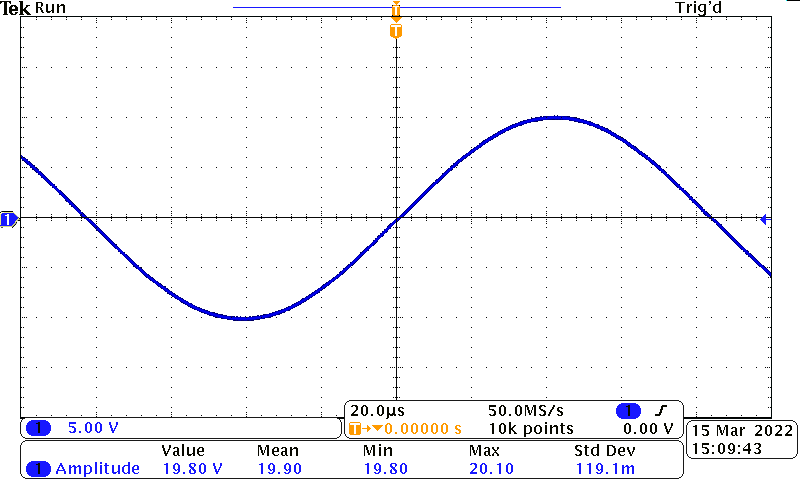
\includegraphics[width=\textwidth]{include/5/ref.png}
		\caption{Pomiar amplitudy odniesienia}
	\end{figure}

	W kolejnym kroku obciążono wyjście generatora za pomocą rezystora nastawnego, który umożliwiał nastawę wartości oporu odpowiadającej znamionowemu oporowi wyjściowego generatora.
	Następnie dostosowano nastawę rezystora \(R_l\) tak aby amplituda napięcia odczytywana w dalszym ciągu na oscyloskopie zmalała około o połowę, do \(U=10.20\)V.
	
	\clearpage
	\begin{figure}[htp]
		\centering
		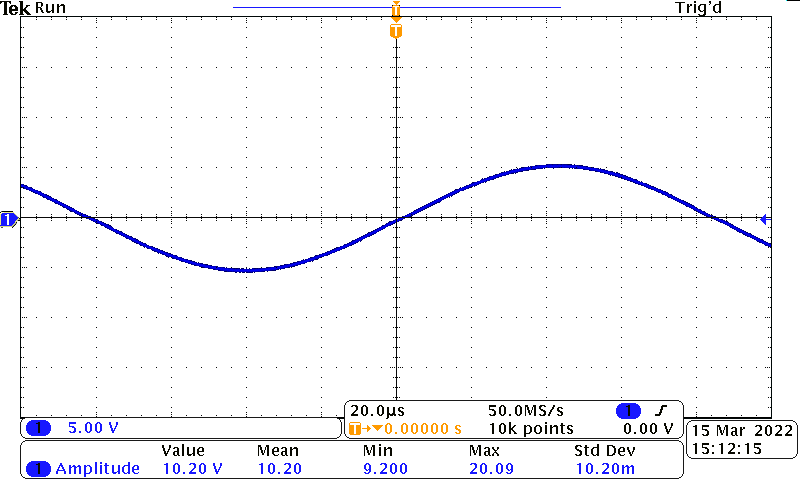
\includegraphics[width=\textwidth]{include/5/60.7R.png}
		\caption{Opór rezystora nastawnego dobrany tak aby amplituda zmalała o połowę względem amplitudy odniesienia}
	\end{figure}

	Zmierzono następnie nastawę rezystora za pomocą omomierza, wyniosła ona \(60.7\Omega\).
	Korzystając z prawa Ohma i zakładając nieskończenie dużą rezystancję wejściową oscyloskopu, rezystancja wyjściowa (wewnętrzna) generatora \(R_w\) jest równa: 
	\begin{align}
		R_w = \biggl(\frac{U_{od}}{U} - 1\biggr)\;R_l = 
		\biggl(\frac{19.90V}{10.20V} - 1\biggr)\;60.7\Omega = 57.7\Omega
	\end{align}

	Odstępstwo od nominalnej wartości \(50\Omega\) może wynikać z niedokładności elementów wchodzących w skład generatora, niedokładności pomiaru oporu rezystora nastawnego lub skończonej rezystancji wejściowej oscyloskopu.

\end{document}